%************************************************
\chapter{The Kerr spacetime}\label{ch:KerrG}
%************************************************

Throughout all the work we will use natural units, so we will set the speed of light ($c=1$) and the universal gravitation constant ($G_N=1$). Notice that in this unit system the dimension of space and the dimension of time are equivalent. Also, the Penrose index notation will be used (the contravariant or covariant character of the tensors is described by the number of super-indexes and sub-indexes respectively). In this chapter we are going to display some interesting and basic features of the Kerr-Spacetime. All this features are well known and can be found with much more detail in the first Chapter of \cite{o1995geometry}. Despite this, we believe it is interesting to make a brief illustrative trip through the behaviors of the Kerr black hole as well as the features of the causal observers moving in the Kerr geometry in a suitable way for any reader with a basic knowledge of differential geometry and general relativity. As any other black hole, the Kerr black hole has an event horizon that prevents that any observer that cross this surface can go back and therefore ``protects'' the singularity. But in the Kerr spacetime the structure of the horizons (there is more than one) is more complicated that in the \gls{SW} geometry or the \gls{RN} geometry because in this case there is also a region called \textit{ergosurface}, in which particles cannot remain static, neither can rotate in the opposite direction of the black hole rotation, i.e. in this region the only allowed movement is to move co-rotating with the black hole. Also, as we will see, the Kerr true singularity cannot be understood in the standard coordinates (which are called \gls{BL} coordinates) and we will have to express the metric in another coordinate system to unveil the true nature of this singularity.

\section{The Kerr metric in Boyer-Lindquist coordinates}
The explicit form of the metric in \gls{BL} coordinates is
 \begin{align*}
 ds^2&=-d\bar{t}^2+ \Sigma \left(\frac{dr^2}{\Delta}+d\theta^2 \right)+(r^2+a^2)\sin^2{(\theta)} d\bar{\phi}^2\\
 &+\frac{2 M r}{\Sigma}(a \sin^2{(\theta)} d \bar{\phi} -d\bar{t})^2
\end{align*}
where
\begin{align}
 \Delta(r)&=r^2-2Mr+a^2\\
 \Sigma(r,\theta)&=r^2+a^2 \cos^2 \theta
\end{align}
The \gls{BL} coordinates are form by the tetrad $\{\bar{t},r,\theta,\phi\}$ which takes values on $\bar{t}\in \mathbb{R}$, $r \in \mathbb{R}^+$ , $\{\theta,\phi \} \in S^1$. The Kerr metric depends on two parameters, $M$ and $a$. If we compare the metric with the far field metric generated by an isolated object we can deduce that these parameters are respectively the mass and the angular momentum per unit of mass of the black hole, both measured at the infinity. Some properties of the Kerr black hole arise from the properties of the metric:
\begin{enumerate}
 \item The Kerr metric is stationary, which means that the metric it does not depend explicitly on the coordinate $\bar t$ that yields the (asymptotic) time..
 \item The Kerr metric is axisymmetric, which means that the metric does not depend on the $\phi$ coordinate.
 \item The Kerr metric is not static because it is not invariant under the time reversal transformation $\bar{t} \rightarrow -\bar{t}$
 \item The Kerr metric is invariant under the transformation
 \begin{align}
  \bar{t} & \rightarrow -\bar{t}\\
  \phi & \rightarrow - \phi
 \end{align}
this can be interpreted as the time reversal of the Kerr metric produces a black hole that is rotating in the opposite direction.
\item Is asymptotically flat, which means that in the limit $r \to \infty$ the Kerr metric becomes the Minkowsky metric in spherical coordinates.
\item In the limit $a \to 0$ the Kerr metric becomes the \gls{SW} metric in Droste coordinates.
\item In the limit $M \to 0$ (but $a \neq 0$) the Kerr metric becomes isometric to the Minkowsky spacetime in spherical coordinates.
\end{enumerate}

\section{Symmetries}

As we notice before, the Kerr metric has two important symmetries because its stationary and axisymmetric. Therefore, the Kerr metric admits two Killing vector fields (to know more about Killing vectors, see \vref{Killingchapter})
\begin{equation}\label{killvec}
 \xi_1= \partial_t \quad \quad \quad \xi_2=\partial_\phi.
\end{equation}
If we name $u^\alpha$ to the geodesics tangent vector, there exist two conserved quantities associated with this Killing vectors:
\begin{align}\label{conserved11}
 -E = u^\alpha {\xi_1}_\alpha \quad \quad \quad L_z=u^\alpha {\xi_2}_\alpha
\end{align}
In the case of timelike geodesic these conserved quantities can be interpreted as the energy per unit of mass of the particle measured at the infinity and the angular momentum per unit of mass measured at the infinity. In the case of null geodesics this interpretation can be maintained if we parametrize the geodesic flow with the affine parameter of the geodesic. In the following, this convention will be maintained. 

\section{The curvature}
  \begin{figure}[htp!]  
\begin{center}
 \centerline{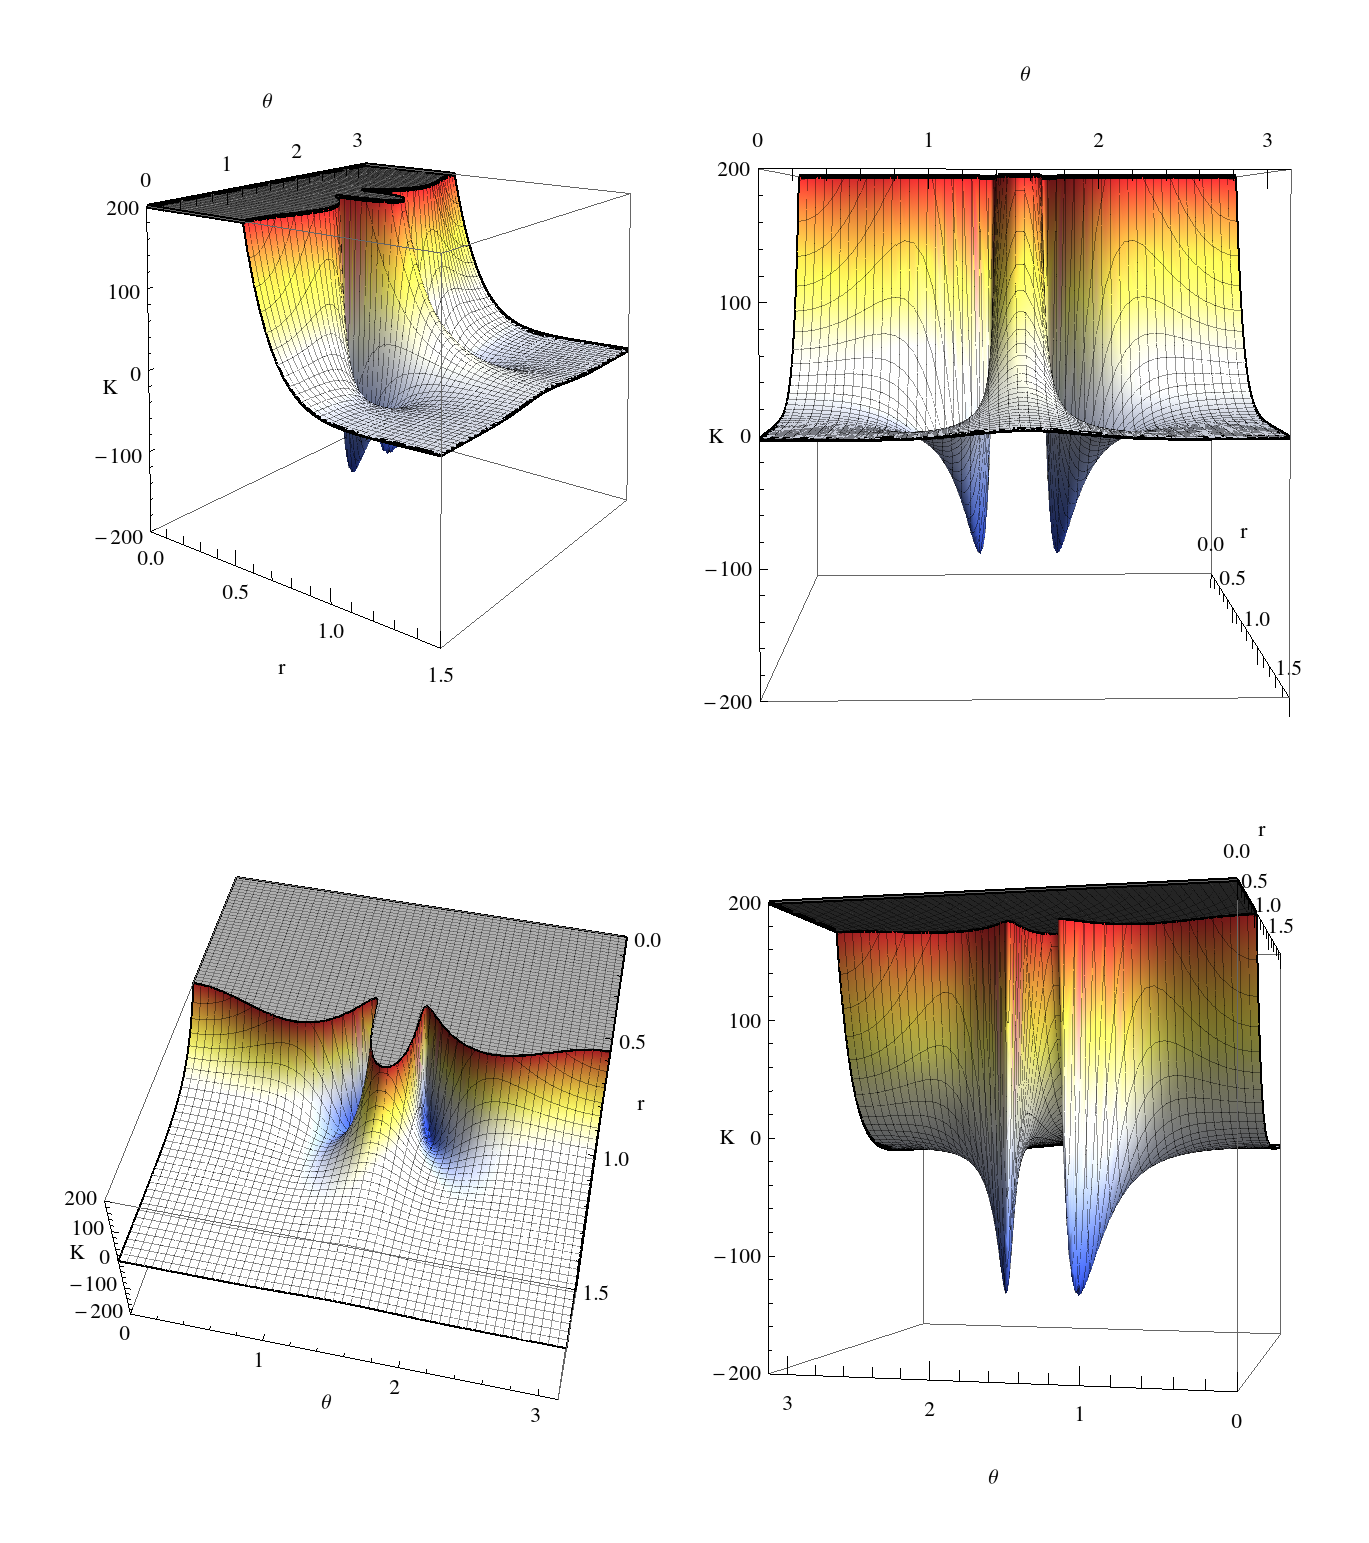
\includegraphics[width=1\textwidth]{img/Chapter0/Kresch.png}}
 \end{center}
 \vspace{-1.5cm}
 \caption{The figure shows the variation of the Kretschmann invariant as a function of the variables $r$ and $\theta$ of the \gls{BL} coordinates. The grey region indicates  the cut-off of the surface which continues to higher values. $M=1$ and $a=0.9$ has been chosen for illustrative purposes.}
 \label{fig:Kresch}
\end{figure} 
The curvature scalar is usually defined by the Riemann scalar
\begin{equation}
 R=Ric^{\alpha}_{\,\alpha}
\end{equation}
where $Ric_{\alpha \beta}=R^\gamma_{\,\alpha \gamma \beta}$ and $R^{\alpha}_{\,\beta \gamma \delta}$ is the Riemann tensor. However the scalar $R$ vanishes because the Kerr solution corresponds to a solution of the vacuum Einstein equations. The Einstein equations without cosmological constant are
\begin{equation}
 Ric_{\alpha \beta}-\frac{1}{2} g_{\alpha \beta} R=T_{\alpha \beta}
\end{equation}
where $T_{\alpha \beta}$ is the Energy-Stress tensor. Taking the trace of the equations we get
\begin{equation}
 -R=T
\end{equation}
where $T=T^\alpha_{\,\alpha}$. As for the vacuum Einstein field equations we have that $T_{\alpha \beta}=0$ then $R=0$ and therefore the curvature scalar does not give any information of the spacetime curvature. But we can construct other invariant quantities with the Riemann tensor. One of the most important ones is the invariant $K=R_{\alpha \beta \gamma \delta}R^{\alpha \beta \gamma \delta}$, which is known as the Kretschmann invariant. As any other invariant, its properties does not depend of the choice of the coordinate system. A direct computation of the Kretschmann invariant in \gls{BL} coordinates gives
\begin{equation}
 K=R_{\alpha \beta \gamma \delta}R^{\alpha \beta \gamma \delta}=\frac{8 \left(6 M^2 \left(-a^6 \cos ^6(\theta )+15 a^4 \cos ^4(\theta )-15 a^2 r^4 \cos ^2(\theta )+r^6\right)\right)}{\left(a^2 \cos ^2(\theta )+r^2\right)^6}
\end{equation}
The variation of $K$ as a function of $r$ and $\theta$ is depicted in \cref{fig:Kresch}. Notice that there exist regions with negative curvature, which means that in this region the Riemann tensor is fundamentally timelike, which can only happen in Lorenzian manifolds. We see that the curvature becomes infinite iff
\begin{equation}
a^2 \cos ^2(\theta )+r^2= 0 \rightarrow r=0 \quad \quad \mbox{and} \quad \quad \theta=\frac{\pi}{2},
\end{equation}
which is the only true spacetime singularity.

\section{Singularities and horizons}

The Kerr metric has some interesting properties that concern spacetime singularities. Some of these singularities are not really there, as they are which is known as \textit{Coordinate singularities}, that are points where the expression of the metric element becomes singular but due to a bad election of the coordinate system. Although this may seem only a problem of the coordinate system, these singularities are much more interesting, because they reveal some interesting causal properties of the Kerr spacetime. We can see that the Kerr metric is singular when
\begin{align}
 \Delta &=0,\\
 \Sigma&=0.
\end{align}
We will name these equations \textit{singularity equations}. The singularities of the first equation (namely $r=r_\pm$) correspond to a pair of \textit{coordinate singularities} as the computation of the Kretschmann invariant $R_{\alpha \beta \gamma \delta}R^{\alpha \beta \gamma \delta}$ (where $R$ is the Riemann tensor) suggests that these points are not truly spacetime singularities and we call them \textit{horizons}. On the other hand the singularity of the second equation is really a spacetime singularity as we have seen in the last section.

The coordinate singularities given by $\Delta=0$ are located at
\begin{equation}
 r=r_\pm=M \pm \sqrt{M^2-a^2}
\end{equation}
When $a^2<M^2$ the two solutions of the singularity equation exist but when $a^2=M^2$ they become one solution as $r_+=r_-=M$. For values of the angular momentum of the black hole that fulfill $a^2>M^2$ there is no real solution to the singularity equation and therefore no horizons exist. In this situation the Kerr solution does not describe a black hole, as the spacetime singularity is not covered by any event horizon, which will lead to paradoxes. This is the reason that all astrophysical processes are believed to lead to black holes with $a^2 \leq M^2$. When $|a|=|M|$ the Kerr spacetime is called \textit{extremal black hole} and for values of $a$ and $M$ such that $|a|>|M|$ the black hole is called \textit{superextreme black hole}. Let us consider now the normal 1-form to the constant-$r$ hypersurfaces which is given in  \gls{BL} coordinates as
\begin{equation}
 n_\alpha=(0,1,0,0)
\end{equation}
By the use of the Kerr metric we can evaluate its norm as
\begin{equation}
 n^\alpha n_\alpha= n^\alpha n^\beta g_{\alpha \beta} = \frac{\Delta}{\Sigma}.
\end{equation}
We can see that on the horizons ($r=r_\pm$) $n^\alpha n_\alpha=0$ which reveal that they are null hypersurfaces, and this is because they are called horizons. The two horizons separate the structure of the spacetime in three regions
\begin{enumerate}
 \item The region in which $r>r_+$. In this region the constant-$r$ surfaces have timelike causal character and as in the limit $r \to \infty$ the metric becomes the Minkowsky metric, we say that this is the exterior of the black hole.
 \item The region in which $r_-<r<r_+$ the constant-$r$ surfaces have spacelike causal character. A deeper analysis of the causal structure tell us that an object that falls through $r=r_+$ can only continue falling until it reaches $r=r_-$. This is the reason we call $r=r_+$ the event horizon.
 \item The region in which $r<r_-$ the constant-$r$ surfaces are timelike again and this is the region that contains the spacetime singularity.
\end{enumerate}
Notice that in the range $a^2 \geq M^2$ the second region does not exist and when $a^2>M^2$ the 1st and 3rd regions are causally connected because there is no horizon that prevent this behavior.

Notice that the spacetime singularity is located at $r=0$ and $\theta=\frac{\pi}{2}$ (but no at $r=0$ and $\theta \neq \frac{\pi}{2}$).This relation has no meaning in spherical-like coordinates (the \gls{BL} coordinates). We need another coordinate system to reveal the true shape and properties of the spacetime singularity. In the next chapter, we will see that in another well-behaved coordinate system, the Kerr singularity happens to be a ring that increases it radius with the value of $a$, being a single point when $a=0$.

\section{ZAMOS}
  \begin{figure}[htp!]  
\begin{center}
 \centerline{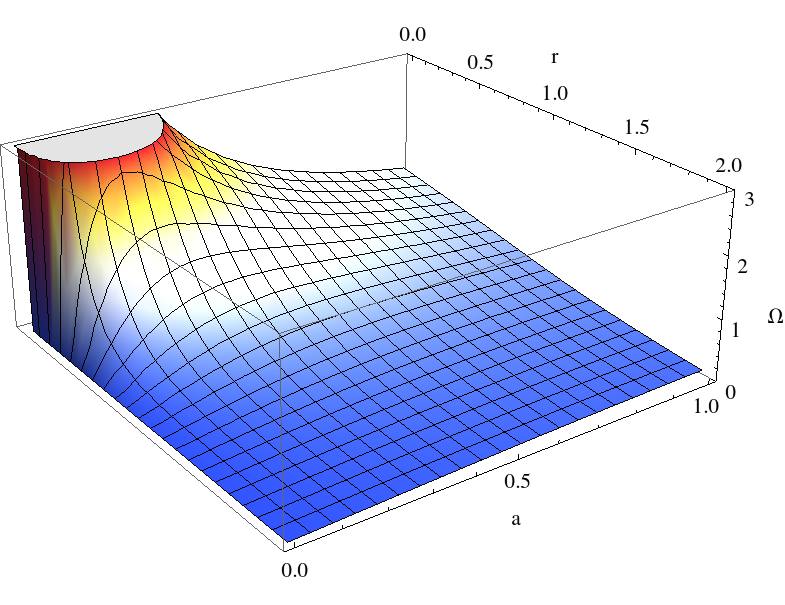
\includegraphics[width=0.8\textwidth]{img/Chapter0/ZAMO.png}}
 \end{center}
 \caption{The figure shows the ZAMO angular velocity $\Omega$ in de equatorial plane ($\theta=\frac{\pi}{2}$). The color is proportional to the value of $\Omega$ (that is in the vertical axis also) and it is only for improve the visualization.}
 \label{fig:ZAMO}
\end{figure} 
We are going to study one of the most popular Kerr features, that is the frame dragging. Remember that a Newtonian observer in a axisymmetric potential (or even an observer in the \gls{SW} or \gls{RN} geometries) in freefall has a radial trajectory if $L_z=0$. This is because the radial velocity is proportional to the angular momentum $L_z$. To study what happens in the Kerr spacetime, let us consider an observer with zero angular momentum. In virtue of \cref{conserved11} we can write
\begin{equation}\label{zamoeq1}
 L_z=u_{\bar{\phi}}=0
\end{equation}
In the literature, this observer is commonly known as \gls{ZAMO}. Notice that the contravariant component of the velocity is
\begin{equation}
 u^{\bar{\phi}}=g^{\bar{\phi} \bar{t}}u_{\bar{t}} \neq 0
\end{equation}
and therefore the \gls{ZAMO} can, in principle, have radial component in the tangent vector and therefore its trajectory will not be a radial movement. From \cref{zamoeq1} we can write
\begin{equation}
 u_{\bar{\phi}}=g_{\bar{\phi} \bar{\phi}}u^{\bar{\phi}} + g_{\bar{\phi} \bar{t}} u^{\bar{t}}=0
\end{equation}
and therefore the angular velocity of the \gls{ZAMO} is given by
\begin{equation}
 \Omega=\frac{u^{\bar{\phi}}}{u^{\bar{t}}}=-\frac{g_{\bar{\phi} \bar{t}}}{g_{\bar{\phi} \bar{\phi}}}=\frac{2 M a r}{(r^2+a^2)^2-a^2 \Delta sin^2\theta}.
\end{equation}
The \cref{fig:ZAMO} shows the behavior of this function in the equatorial plane (the behavior is similar for other values of $\theta$). Notice that as the denominator is always positive then
\begin{equation}
 sign(\Omega)=sign(M a)
\end{equation}
and therefore the \gls{ZAMO} rotates in the same direction as the black hole. We conclude two important results:
\begin{itemize}
 \item Observers with zero angular momentum cannot move in radial movements (straight lines) .
 \item An observer which approaches a Kerr black hole with zero angular momentum is dragged by the gravitational force of the black hole and the only movement allowed is rotate in the same direction as the black hole.
\end{itemize}
  \begin{figure}[htp!]  
\begin{center}
 \centerline{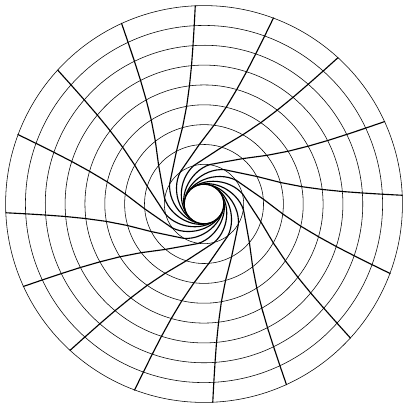
\includegraphics[width=0.6\textwidth]{img/Introd/Dragg.png}}
 \end{center}
 \caption{Frame dragging in the Kerr spacetime. }
 \label{fig:Dragg}
\end{figure} 
The effect of the frame dragging over the \gls{ZAMO}s can be visualized in \cref{fig:Dragg}, where we can see how the trajectories with $L_z=0$ (that are straight lines in the infinity as $\lim_{r\to\infty} \Omega=0$) are dragged by the Kerr black hole. We will see that the frame dragging is even more strong and complex that that and has a very important role in what is known as the ergoregions.

\section{The ergosphere}

In the \gls{SW} geometry it is known that the Killing vector $\partial_{\bar{t}}$ is timelike outside the even horizon (remember that in the \gls{SW} geometry there is only one horizon), null over the horizon and spacelike inside the horizon. That is why it is said that inside the horizon the coordinate $\bar{t}$ measures space while the coordinate $r$ measures time. as the \gls{SW} singularity is located at $r=0$ and as inside the horizon $r$ measures time, its said that the \gls{SW} singularity its not a place but a time: \textit{The singularity is not there but it is tomorrow}. This can be easily understood if you think that tomorrow the universe reachable by you is supposed to disintegrate and disappear. This is what "hitting" the \gls{SW} singularity is not a "place", it is everywhere in the future. However, in the Kerr spacetime the singularity is located at $r=0$, and in this region $r$ is a spacelike coordinate and therefore the singularity in really a ''place'', not a moment in time. In the Kerr geometry, the points where the Killing vector changes its spacetime causal character (timelike, null or spacelike) do not match with the singularities (coordinate singularities) of the metric. As the causal character of the Killing vector is given by$g(\partial{\bar{t}},\partial{\bar{t}})=g_{tt}$ we can see where the component $g_{tt}$ changes its sign. We write
\begin{equation}
 g_{tt}=-1+\frac{2M r}{\Sigma}=\frac{r^2-2M r+a^2 \cos^2 \theta}{\Sigma}=0.
\end{equation}
This equation has two solutions
\begin{equation}
 r_{E\pm}=M \pm \sqrt{M^2-a^2 \cos^2\theta}.
\end{equation}
These two solutions are known as the \textit{ergosurfaces} and also as the \textit{infinity redshift surfaces}. The reason of the second name is that if we think in a light source located on a point $p_s$ that emits a light pulse with frequency $\nu_s$ it will be observed with frequency
\begin{equation}
 \nu_{\text{obs}}=\sqrt{\frac{g_{tt}(p_s)}{g_{tt}(p_\text{obs})}}  \nu_s
\end{equation}
(where $ \nu_{\text{obs}}$ is the frequency measured by an observator located at the point $p_\text{obs}$) and therefore the observed frequency is $ \nu_{\text{obs}}=0$ if the light pulse is emitted from $p_s=r_{E \pm}$ because $g_{tt}(r_{E \pm})=0$. Let us call $\mathcal{I}=[r_{E-},r_{E+}]$, the interval between the two ergosurfaces. Notice that the two horizons are always in this interval ($r_\pm \in \mathcal{I}$) as
\begin{equation}
 r_- \leq r_{E-} \leq r_{E+} \leq r_+.
\end{equation}
  \begin{figure}[htp!]  
\begin{center}
 \centerline{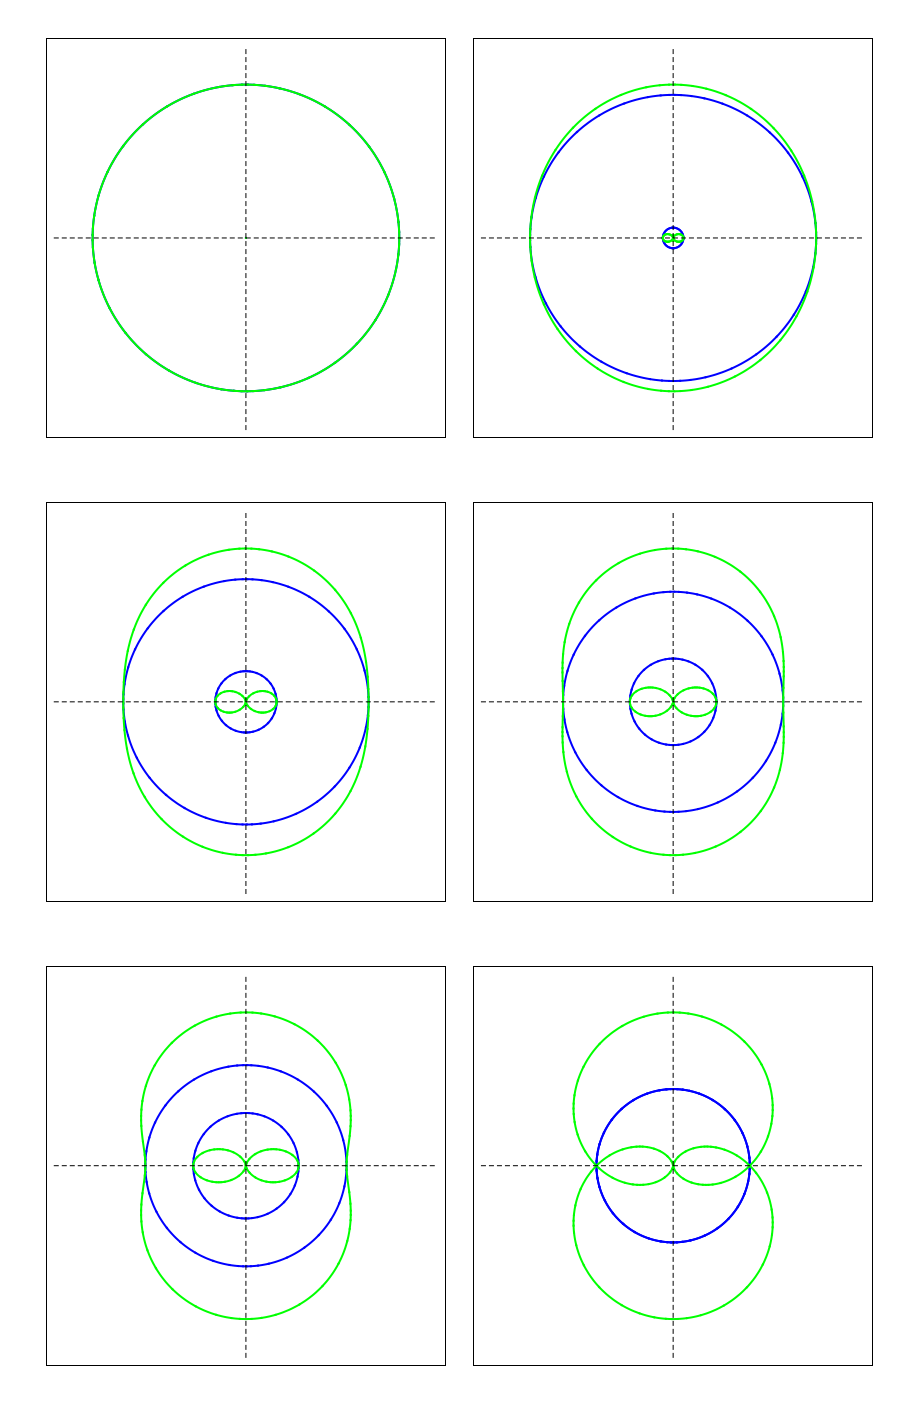
\includegraphics[width=0.95\textwidth]{img/Chapter0/erg.png}}
 \end{center}
 \vspace{-1.5cm}
 \caption{Schematic location of the horizons, ergosurfaces, and curvature singularity in the side view of the Kerr Spacetime in \gls{BL} coordinates as a function of the parameter $a$. The images correspond to (from left to right and from top to bottom) $a=0$,$a=0.5$,$a=0.8$,$a=0.9$,$a=0.95$,$a=1$. The green surfaces are the outer and inner ergosurfaces and the blue curves represent the inner and outer horizon. Notice that the singularity is at the center of the image ($r=0$ $\theta=\frac{\pi}{2}$). For simplicity $M=1$ is chosen.}
 \label{fig:ergo1}
\end{figure} 
In \cref{fig:ergo1}, a schematic image of the horizon and ergosurfaces is displayed. Given these results, we have have that $g_{tt}<0$ iff $r \notin \mathcal{I}$ and $g_{tt}>0$ iff $r \in \mathcal{I}$. Therefore, there is a region between the outer horizon and the outer ergosurface where $g_{tt}>0$ (this does not happen in the \gls{SW} spacetime). This region is known as the \textit{ergoregion} and $r=r_{E+}$ is called  \textit{ergosphere}. Its very important that the ergoregion exists outside the outer horizon, because this fact allows a geodesic that comes from the asymptotically flat region enter the ergoregion and escape to the asymptotically flat region again (without being trapped by the black hole as the geodesic does not cross the even horizon). As $g_{tt}>0$ in this region, the Killing vector becomes spacelike. Some strange features happen in this region. First of all, as the conserved quantity of the $\partial_{\bar{t}}$ Killing vector is $ u^\alpha {\xi_1}_\alpha=-E$ and as $\xi_1$ is spacelike, $E$ can be negative as well. Negative energies are only allowed inside the horizon in the \gls{SW} geometry, as in the \gls{RN} geometry (that is the \gls{SW} spacetime with charge in the source of the gravitational field). The main strange feature is that there is no stationary observers allowed in the ergoregion. An stationary observer is an observer which does not see the metric change in its motion. For example, a observer in $\partial_t$, which is an observer that does not change the coordinates $\{r,\theta,\phi\}$ (and therefore its tangent vector must be proportional to $\partial_{\bar{t}}$) is an example of a stationary observer. As stationary observers does not see the metric change in its motion, and we know that the metric does not change along the trajectories of the Killing vectors, the tangent vector to the geodesic of the stationary observer must be a Killing vector, i.e. a linear combination of the independent Killing vector fields in \cref{killvec}. As the observers in the spacetime must move along causal timelike curves ($u^\alpha u_\alpha =-1$, where $u^\alpha$ is the tangent vector to the trajectory) we can see that observers in $\partial_t$ (those whose tangent vector is proportional to $\partial_{\bar{t}}$) are not allowed in the ergoregion because in this region $\partial_{\bar{t}}$ is spacelike and therefore only stationary observers whose tangent vector is a linear combination of the two Killing vectors are allowed. To understand what this means we are going to compute the unitary tangent vector of a general stationary observer as
\begin{equation}
 u^\alpha=\frac{\partial_{\bar{t}}+\omega \partial_\phi}{|\partial_{\bar{t}}+\omega \partial_\phi|}=(u^t,0,0,u^\phi)=u^t(1,0,0,\omega),
\end{equation}
where we have defined $\omega$ as
\begin{equation}
 \omega= \frac{d \phi}{d \bar{t}}=\frac{u^\phi}{u^t},
\end{equation}
to be the constant angular velocity of the observer. As we see, the trajectory of the observer has constant $r$ and $\theta$ coordinates and can only move along a circle with angular velocity $\omega$. Observer's tangent vectors must fulfill
\begin{equation}\label{conditionob}
 u^\alpha u_\alpha=(u^t)^2 \left( g_{tt}+ 2 \omega g_{t \phi}+ \omega^2 g_{\phi \phi} \right) =-1 \rightarrow  g_{tt}+ 2 \omega g_{t \phi}+ \omega^2 g_{\phi \phi}<0.
\end{equation}
To understand this equation, let us solve
\begin{equation}
  g_{tt}+ 2 \omega g_{t \phi}+ \omega^2 g_{\phi \phi}=0.
\end{equation}
The solutions of this equation are
\begin{equation}
 \omega_{\pm}=\frac{-g_{t\phi} \pm \sqrt{g_{t \phi}^2- g_{tt} g_{\phi \phi}} }{g_{\phi \phi}}.
\end{equation}
Notice that the discriminant of the equation is $g_{t \phi}^2- g_{tt} g_{\phi \phi}=\Delta \sin^2 \theta$ and therefore this equation has no real solutions for $\Delta <0 $ which implies $r_-<r<r_+$. This has the meaning that no stationary observers are allowed when  $r_-<r<r_+$ . Outside the outer horizon $r>r_+$ we have that $\Delta>0$ and the inequality \cref{conditionob} is satisfied when
\begin{equation}
 \omega_- <\omega <\omega_+.
\end{equation}
As we have that in the ergosphere ($r=r_{E+}$) $\omega_-(r=r_{E+})=0$ as $g_{tt}=0$ in this surface, then for $r \geq r_{E+}$ we will have $\omega_- \leq 0$ and the stationary observer can spin contra-rotating with the black hole ($\omega<0$) or co-rotating with the black hole ($\omega>0$). For $r_+<r<r_{E+}$ we have that $\omega_->0$ and therefore the observer can only rotate co-rotating with the black hole. This can be summarized as
\begin{enumerate}
 \item There is no stationary observer in the region $r_-<r<r_+$ .
 \item When a particle is in the ergoregion ($r_+<r<r_{E+}$, it can only move spinning co-rotating with the black hole and it cannot remain static (constant $\{r,\phi,\theta\}$ at the same time).
 \item Outside the ergoregion ($r \geq r_{E+}$ ) particles can move co-rotating or contra-rotating and observers in $\partial_t$ are allowed.
\end{enumerate}

Notice that as only photons (null causal curves) are allowed to move in the outer horizon $(r=r_+)$ and in this region $\omega_-=\omega_+$, then the only angular velocity of a null stationary observer is $\omega=\omega_\pm=\frac{2 M a r_+}{(r_+^2 + a^2)^2}=\frac{a}{r_+^2+a^2}=\Omega$, which is also the \gls{ZAMO} angular velocity. As this angular velocity is constant we can say that the black hole \textit{rotates rigidly}. This is because the angular velocity of the only curves that can remain in $r=r_+$ (that are null causal geodesic with its tangent vector given by $u^\alpha=(u^t,0,0,u^\phi)$ with $u^\alpha u_\alpha=0$) does not depend on the value of any coordinate.

\section{The Penrose process}
  \begin{figure}[htp!]  
\begin{center}
 \centerline{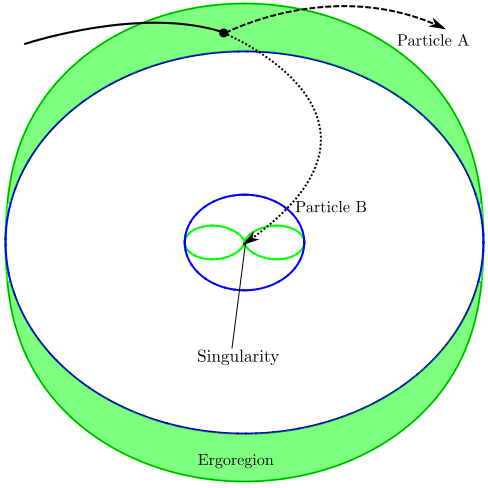
\includegraphics[width=0.4\textwidth]{img/Chapter0/Penrose.png}}
 \end{center}
 \caption{The figure shows the Penrose process in \gls{BL} coordinates. The green curves represent the inner and outer ergosphere and while the blue ones are the outer and inner horizons. Remember that in this coordinate system the singularity is located at $r=0$. For illustrative purposes $a=0.8$ and $M=1$ is chosen.}
 \label{fig:penroprocc}
\end{figure} 
The ergosphere has another very interesting feature: The Penrose process. As we have seen, the energies in the ergosphere can be negative $(E<0)$ as the Killing is spacelike in this region. Let us consider a particle that follows a geodesic that comes from the asymptotically flat region and then enters the ergosphere. Under some specific circumstances circumstances can decay into two particles A and B between the ergosphere and the outer horizon (this region is called ergoregion). The decay can be done in such a way that the particle B falls into the singularity, passing through the outer horizon, the inner horizon and the inner ergosphere and the particle B escapes to the asymptotically flat region. If the ingoing particle has energy $E$ and the two particles have energies $E_A$ and $E_B$ respectively, the global energy conservation allow us to write
\begin{align}
E&=E_A+E_B,\\
 E_\text{Kerr initial} + E&= E_\text{Kerr final}+E_A.
\end{align}
Particle B, crossing the event horizon, has a negative energy because within the ergosphere, the Killing vector $\partial_{\bar{t}}$ is spacelike and negative energies are allowed (remember that $g(\partial_t,u^\alpha)=-E0$, where $-E<0$ in the ergoregion). Then, as the total energy is conserved, the black hole absorbs a negative energy. The particle A that goes to infinity will gain that amount of energy because of the energy conservation $E_A>E$. Notice that as this process occurs at $r>r_+$ the particle A can return to the asymptotically flat region with more energy and therefore this act like a ''generator'', because we sent a particle with energy $E$ and we have gained a particle with energy $E_A>E$. The global result is that the Kerr black hole decelerates its rotation since it has absorbed negative energy. Blandford and Znajek (1977) suggested that the Penrose process could be a characteristic feature of Kerr black holes surrounded by a accretion disk containing a strong magnetic field. If this magnetic fields penetrates the ergoregion, then it could be a realistic source of electrons and positrons (created in pairs) which could start the Penrose process. This scenario involves that one of the particles end up with negative energy and falls into the black hole, while the other escapes to the asymptotically flat region. This second particle might form the characteristic energetic jets of charged particles that are known to be emitted from Kerr black holes, especially in quasars. By this process, quasar jets are powered by the energy that they extract from the Kerr black hole.


